\documentclass[11pt]{article}

%Don't change any thing before \begin{document}
%In fact if you use sth fancy, you might need
%to add more packages, or macros.
\usepackage{amssymb,amsmath}
\usepackage{times,psfrag,epsf,epsfig,graphics,graphicx}
\usepackage{algorithm}
\usepackage{algorithmic}


\begin{document}
\date{}

\title{CSCI 338: Assignment~1}

\author{Your Name Here}

%\author{Peter Pan \and John Paxton \and  Binhai Zhu}
%If you have collaborators in later assignments

\maketitle


\section*{Problem 1}

Your solution to Problem 1 goes here. Remember, \emph{each problem} should be
starting on a new page.

If the problem has subparts, it will be convenient to use the enumerate
environment:
\begin{enumerate}
    \item {\bf TODO}: give the solution to subproblem (1) here.
    \item \underline{More TODO}: give the solution to subproblem (2) here.
\end{enumerate}

If for whatever reason enumerate will not suffice (perhaps if your answers are
getting rather long), then use subsection*:

%If you want to split the assignment questions to a new page, uncomment the next line
%\newpage

\subsection*{Problem 1(a)}
TODO: give solution here.


\subsection*{Problem 1(b)}
TODO: give solution here, etc.


And the second problem should go on a fresh page.
\newpage

%Note the difference between section and section*
\section{Problem 2}

Well, this looks weird initially, but you will like it when you have to deal
with mathematical formulas, like $a^2+b^5=c^2$ and $(c>0)\rightarrow [c^{x}>2020]$ implies $a$ and $b$ are good guys, $c$ is horrible and $x$ is a disaster..
\newline

Or, what is even more complex:
 the $p$-{\em Wasserstein} distance is defined as
$$W_p(D_k(U),D_k(V))=\left( \inf_{\phi}\sum_{x\in D_K(U)}\|x-\phi(x)\|^p_{\infty}\right)^{1/p},$$ 
where $\phi:D_k(U)\rightarrow D_k(V) \mbox{~is~a~bijection}.$
This hard to do with Word.
\newline

If you don't need a line, but being cautious so that you don't want to delete
the line, just comment it out using \% at the beginning of that line.
\newline

\begin{figure}[htbp]
\begin{center}
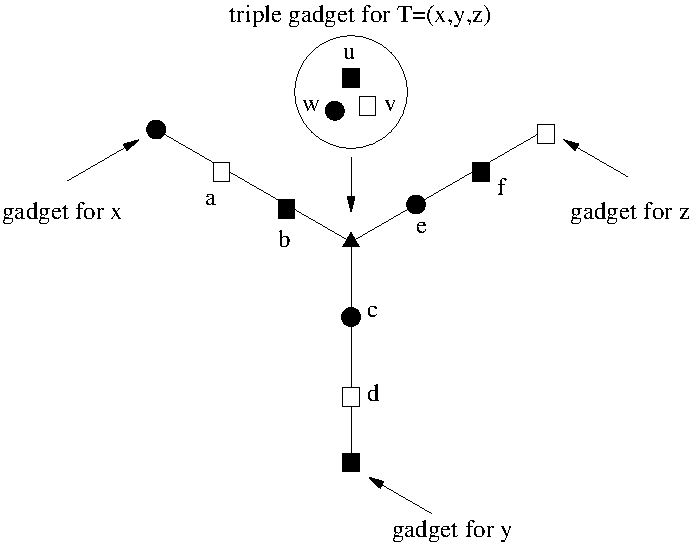
\includegraphics[scale=0.55]{fig8.pdf}
\end{center}
\label{fig1}
\caption{\bf The triple gadget for $T=\langle x,y,x\rangle$ (represented as $\blacktriangle$, which is really putting three element points $u,v$ and $w$ in distinct colors on a grid point). If the triple $\langle x,y,z\rangle$ is not selected in the final solution, then the optimal local clusters would be $(a,b,w)$, $(c,d,u)$ and $(e,f,v)$. A different set of local clusters, e.g., $(a,b,c)$, $(d,e,f)$ and $(u,v,w)$ would incur a larger cost.}
\end{figure}

Besides dealing with math formulas, one of the advantage of using Latex to do
your assignments is that making changes are a whole lot easier. Imagine that you
do the assignment by hand, if you finish a half page and then find that some
serious mistakes are made --- you would have no choice but re-writting the
half page by hand again (even some part of it does not contain any mistake or error). With Latex, this is not a problem at all!
\newline

You could also include a figure (in either .pdf or .eps format). In Figure 1,
I include a figure named {\bf fig8.pdf} in the same directory as the HW-XX.tex file.

\section*{Problem 3}

Prove that if $x$ and $y$ are both even integers, then
$$z=\frac{37x-11y}{2}$$
is also an even integer.
\newline

\noindent
{\bf Proof}: By assumption, if $x$ and $y$ are both even integers,
then we could rewrite $x=2a$, $y=2b$ where $a,b$ are both integers.
Then,
$z=\frac{37x-11y}{2}=\frac{74a-22b}{2}=37a-11b,$
which must also be an integer.

%many people like using a \Box at the end of a proof
$\hfill \Box$
\end{document}

